\pdfdecimaldigits=6
\documentclass{article}
\usepackage[paperwidth=444.916301bp,paperheight=196.423500bp,margin=0bp]{geometry}
\usepackage{graphicx,tikz,helvet,fix-cm}
\pagestyle{empty}
\setlength{\parindent}{0pt}
\begin{document}
\noindent\begin{tikzpicture}[x=1bp,y=1bp,baseline=0bp]
\path[use as bounding box] (0,0) rectangle (444.916301,196.423500);
\node[overlay,anchor=south west,inner sep=0pt,outer sep=0pt] at (0,-0.0023) {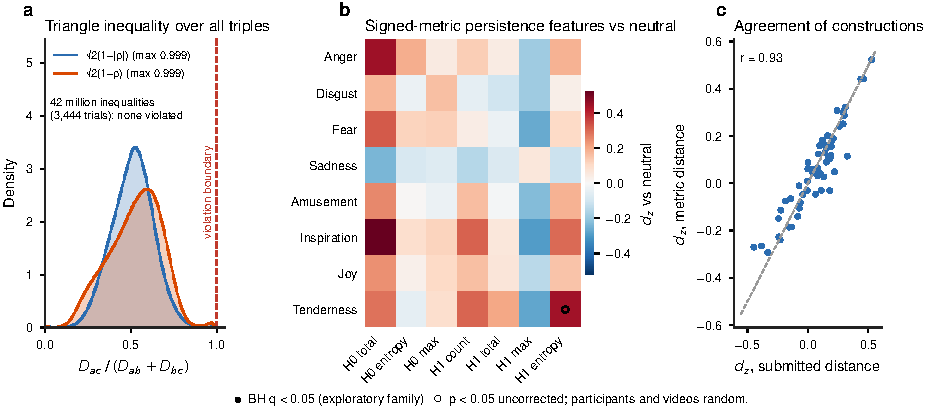
\includegraphics{original_S5.pdf}};
% Replace only two vector axis labels. Coordinates are measured from original PDF.
\fill[white] (349,12.4235) rectangle (427,26.4235);
\fill[white] (320.2,77.0235) rectangle (331.5,138.2235);
\node[inner sep=0pt,font=\sffamily\fontsize{6.4}{7}\selectfont] at (387.8,19.8) {$d_z$, absolute-correlation distance};
\node[inner sep=0pt,rotate=90,font=\sffamily\fontsize{6.4}{7}\selectfont] at (326.1,108.4) {$d_z$, signed-correlation distance};
\end{tikzpicture}
\end{document}
